%نام و نام خانوادگی:
%شماره دانشجویی: 
\مسئله{}
در ارتباط با رابط کاربری و تجربه‌ی کاربری:
\begin{enumerate}[a)]
	\item 
تفاوت رابط کاربری \footnote{\lr{User Interface}} و تجربه‌ی کاربری \footnote{\lr{User Experience}} چیست؟
	\item 
پنج مورد از نقاط قوت و پنج مورد از نقاط ضعف در طراحی رابط و تجربه‌ی کاربری سامانه‌ی آموزش دانشگاه را بیان کنید.‌
\end{enumerate}

\پاسخ{
\begin{enumerate}[a)]
	\item 
تفاوت اصلی این دو در تمرکز اصلی‌شان و نحوه‌ی برقراری ارتباط کاربر با آن‌ها است که درادامه به تفصیل درموردشان صحبت می‌کنیم.
	
رابط کاربری درمورد طراحی، معماری اطلاعات و بخش‌های بصری یک محصول مانند صفحات، دکمه‌ها، رنگ‌‌ها و منوها است که کاربر به هنگام استفاده از محصول مستقیما با آن‌ها تعامل می‌کند. تمرکز رابط کاربری روی بهینه‌سازی این ارتباط و کیفیت محصول است و تنها درمورد محصولات دیجیتال به کار می‌رود. می‌توان گفت که رابط کاربری بخشی از تجربه‌ی کاربری را تشکیل می‌دهد (البته نه به صورت کامل).

تجربه‌ی کاربری مفهومی کلی و انتزاعی است که درمورد تجربه‌‌ی کاربر از قبل تا بعد از خرید محصول به‌کار می‌رود. تجربه‌ی کاربری روی این تمرکز می‌کند که محصول قابل استفاده (Functional) ، در دسترس و کاربرپسند \footnote{User-friendly} باشد. این مفهوم را می‌توان هم درمورد محصولات دیجیتال و هم غیردیجیتال استفاده کرد. برای فراهم کردن تجربه‌ی کاربری خوب باید نیازها، مشکلات‌ و اهداف مشتریان را درک کرد و محصولی تولید کرد که این نیازها را برآورده کند و کار کردن با آن لذت‌بخش و آسان باشد. تجربه‌ی کاربری علاوه بر رابط کاربری و بخش‌هایی از محصول که کاربر با آن‌ها در ارتباط است، نحوه‌ی ارتباط این بخش‌ها بایکدیگر و انتقال کاربر بین آن‌ها را هم دربر می‌گیرد.

برای شفاف‌تر شدن تفاوت بین این دو از یک مثال استفاده می‌کنیم. فرض کنید که در یک کافه قهوه سفارش می‌دهید. در این صورت قاشق، شکر و مواد دیگری که همراه با قهوه به شما تحویل داده‌می‌شوند مربوط به تجربه‌ی کاربری هستند و هدف‌شان بهتر کردن تجربه‌ی شما و برآورده کردن تمامی نیازهایتان است. درکنار آن رنگ فنجان، قاشق و طرح میزها مربوط به رابط کاربری هستند و به ایجاد لذت بصری کمک می‌پردازند. 
\begin{figure}[h]
	\centering
	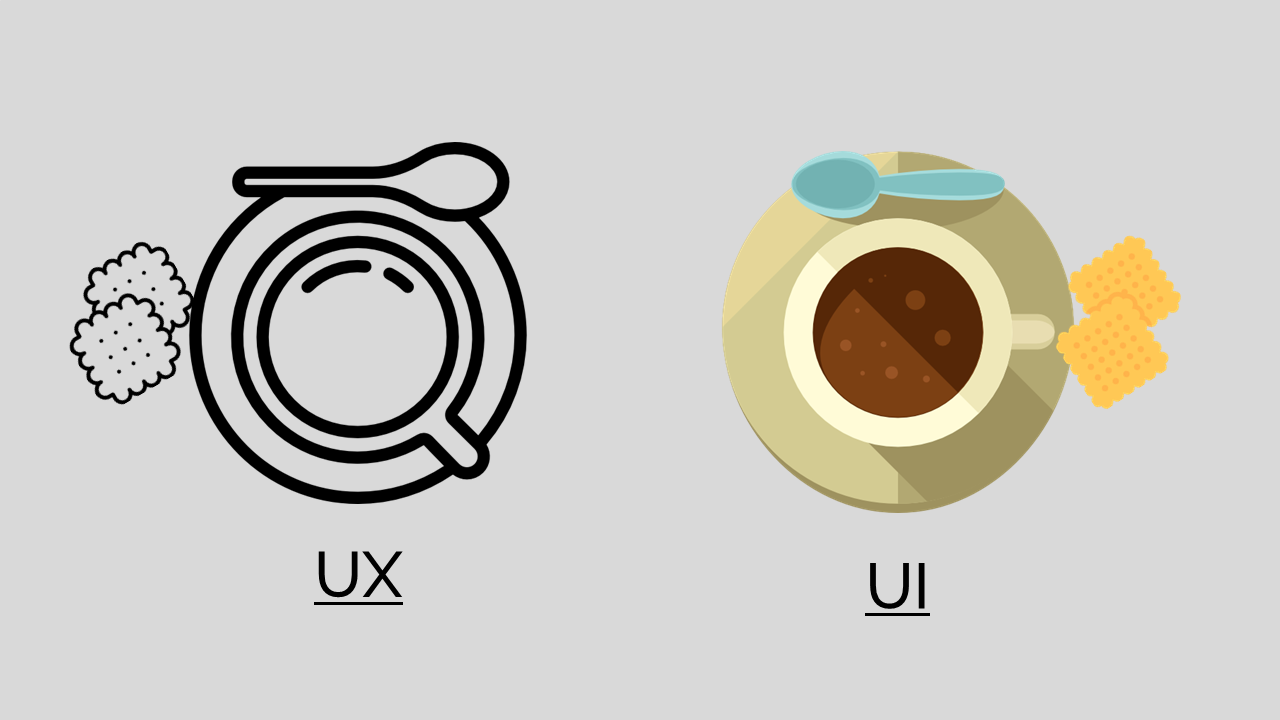
\includegraphics[scale=0.32]{figs/6_1}
	\caption{تفاوت رابط کاربری و تجربه‌ کاربری در مثال کافه}
\end{figure}
\newpage
تفاوت‌های این دو مفهوم به خلاصه در جدول زیر نیز آورده‌شده‌اند:
\begin{center}
    \begin{tabular}{ | r | p{8cm} |}
    \hline
   رابط کاربری & تجربه کاربری \\ \hline
   دید جزئی به محصول & دید کلی به محصول \\ \hline
  جنبه‌های ملموس و قابل دیدن طراحی & جنبه‌های انتزاعی طراحی \\ \hline
    محصول چگونه به‌نظر می‌رسد & استفاده از محصول چه حسی در کاربر ایجاد می‌کند \\ \hline
    بعد بصری تجربه‌ی کار با محصول & تمامی ابعاد تجربه‌ی کار با محصول \\ \hline
    تمرکز روی طراحی سطوح تعامل کاربر  & تمرکز روی تشخیص نیازمندی‌های کاربر و ارائه‌ی راه‌حل‌های ساختاری \\ \hline
  تمرکز روی طراحی محصول نهایی & تمرکز بر مراحل ایده‌پردازی، توسعه و ارائه محصول و تجزیه و تحلیل \\ \hline
    محصولات دیجیتال &  محصولات دیجیتال و غیردیجیتال \\ \hline
    
    \end{tabular}
\end{center}

درنهایت باید تاکید کرد که رابط کاربری و تجربه‌ی کاربری مکمل یکدیگر هستند و هردو برای تولید یک محصول رضایت‌بخش ضروری‌اند و نمی‌توان یکی را به دیگری برتری داد.
	\item 
	نقاط قوت و  ضعف در رابط کاربری و تجربه‌ی کاربری
\href{https://edu.sharif.edu/}{سامانه آموزش دانشگاه}
در ادامه آورده‌شده‌اند.

 \textbf{نقاط قوت}:
\begin{itemize}
\item \textbf{ارائه‌ی واسط کاربری در چهار رنگ متفاوت}:
هر کاربر می‌تواند بنابر سلیقه‌ی خودش از بین رنگ‌های آبی تیره، آبی روشن، قرمز و بنفش یکی را انتخاب کند تا واسط کاربری با آن رنگ نمایش داده‌شود. همچنین بااستفاده از این ویژگی، افرادی که کوررنگی دارند می‌توانند واسط کاربری را به رنگی که قابل‌دیدن است تغییر دهند.
\item \textbf{دسته‌بندی بخش‌های مختلف سایت تحت شش عنوان اصلی}:
منوهای سایت به شکل یک لیست بلند و کلی آورده‌نشده‌اند بلکه به شش دسته‌ی اصلی با موضوعات امور ثبت‌نام و ترمیم، خدمات آموزشی، امور کارنامه، امور پذیرش و مطلوبات کاربر تقسیم شده‌اند. به همین دلیل کاربر نیازی نیست که هربار تک تک منوهای سایت را جستجو کند و  کافی‌است منوهایی که تحت موضوع اصلی مرتبط با خواسته‌اش هستند را بررسی کند. بطور مثال اگر کاربر بدنبال دریافت کارنامه است، باید به بخش امور کارنامه مراجعه کند و منوی مربوطه را انتخاب کند.
\item \textbf{ارائه‌ی اکثر خدمات آموزشی به صورت آنلاین}:
با شیوع کرونا، به سامانه‌ی آموزش بخش‌هایی مانند ورود اطلاعات واکسیناسیون، درخواست لباس جشن فارغ‌التحصیلی و ارسال تصویر مدرک به آموزش اضافه شد. پس از این تغییرات سامانه‌ی آموزشی اکثر خواسته‌های آموزشی کاربران را پوشش می‌دهد و نیازی به مراجعه‌ی حضوری به آموزش دانشگاه نیست. در موقعیت‌های پیش‌بینی نشده‌ی دیگر هم سامانه به‌روزرسانی می‌شود و گزینه‌های جدید به آن افزوده می‌شوند تا دانشجویان بتوانند کارهای ضروری خود را از راه دور انجام دهند.
\item \textbf{طراحی مینیمالیستی}:
در صفحات سامانه‌ی آموزشی عناصر غیرضروری آورده‌نشده‌اند و بخش زیادی از صفحات خالی است. به همین علت است که کاربر با ورود به هر بخش از سامانه، روی متن‌ها و فرم‌های موجود تمرکز می‌کند و بلافاصله هدف آن بخش از سامانه را متوجه می‌شود. به‌این شکل از گیج شدن کاربر جلوگیری می‌شود.
\item \textbf{انسجام بین بخش‌های سایت}:
طراحی دکمه‌ها، فونت و اندازه‌ی متن‌ها، رنگ متن‌ها و همچنین زبان و اصطلاحات به‌کار برده‌شده در بخش‌های مختلف سایت منسجم و مشابه هستند. بطور مثال برای نمایش متن‌های مهم در همه‌جا از رنگ قرمز استفاده‌شده‌است و یا عناوین و متن‌ها با کلمات ساده و روزمره نوشته‌شده‌اند.
\item \textbf{قابل اعتماد}:
سامانه‌ی آموزشی از معتبرترین منابع خبری برای دانشجویان دانشگاه صنعتی شریف است و دانشجویان می‌دانند که درصورتیکه از طریق سامانه درخواستی بدهند، این درخواست تنها توسط افراد مسئول مشاهده می‌شود و همچنین اگر پاسخی دریافت کنند، آن پاسخ قابل اعتماد است و می‌توانند به آن ارجاع بدهند. درنظر گرفتن نقش‌های مختلف برای کاربران و تعیین سطح دسترسی برای هرنقش را می‌توان یکی از عوامل قابل اعتماد بودن سامانه آموزشی دانست. 
\end{itemize}
\textbf{نقاط ضعف}:
\begin{itemize}
\item \textbf{سرعت پایین}:
در زمان‌هایی مانند بازه‌ی ثبت‌نام و ترمیم که سامانه با حجم زیادی از درخواست‌ها روبرو می‌شود، سرعت بارگذاری سامانه و رسیدگی به درخواست‌ها به‌شدت پایین می‌آید. درنتیجه کاربران باید مدت زمان زیادی را صرف کنند تا بتوانند از قابلیت‌های سامانه استفاده کنند. 
\item \textbf{استفاده از فونت نامناسب}:
فونتی که برای متن‌های سامانه به‌کار رفته‌است، جلوه‌ی بصری ندارد. همچنین اندازه‌ی نوشته‌ها کوچک است و امکان تغییر دادن آن برای خوانایی بیشتر وجود ندارد.
\item \textbf{مشخص نبودن وضعیت کنونی سامانه}:
در سامانه مواردی همچون تغییر رنگ دکمه‌ها به هنگام قرار گرفتن نشان‌گر روی آن‌ها و یا نمایش متن درهنگامی که سایت درحال انجام یک عملیات است، پیاده‌سازی نشده‌اند. به‌همین دلیل کاربر نمی‌تواند مطمئن باشد که درخواستش درحال انجام است و یا کلا ثبت نشده‌است. بطور مثال برای ‌بارگذاری فرم در سامانه تنها یک دکمه‌ی ذخیره وجود دارد که پس از کلیک روی آن هیچ نشانه‌ای از اینکه سامانه درحال ذخیره‌ی فرم است یا نه، دیده نمی‌شود. یا در بازه‌ی ثبت‌نام کاربران باید نام درس‌ها را وارد کنند و منتظر ثبت آن‌ها بشوند. اما گاهی سامانه این درخواست را کلا دریافت نکرده‌است و کاربر چون متوجه نشده‌است، زمانی طولانی را منتظر نتیجه‌ی عملیات شده‌است.
\item \textbf{نداشتن گزینه‌ی جستجو}:
یکی از پرکاربردترین بخش‌های هرسایتی، قابلیت جستجو است. این قابلیت به‌ افرادی که آشنایی زیادی در کار با سایت ندارند و یا می‌خواهند به سرعت به یک بخش سایت دسترسی پیدا کنند، کمک می‌کند. اما درحال حاضر سامانه‌ی آموزشی گزینه‌ی جستجو ندارد و کاربر باید به صورت دستی صفحات را جستجو کند.
\item \textbf{نداشتن دسترسی به سامانه از خارج ایران}:
آی‌پی‌های خارجی به سامانه آموزش دسترسی ندارند. این درحالی‌است که سامانه آموزشی باید به دانشجویانی که خارج از کشور هستند کمک کند تا کارهای ضروری خود را به صورت آنلاین انجام دهند.
\item \textbf{نداشتن گزینه کیف پول}:
بعضی از عملیات‌ها (مانند دریافت کارنامه‌ی غیررسمی) نیازمند پرداخت مبلغی به‌صورت آنلاین هستند. با این وجود کاربر نمی‌تواند از قبل مبلغی را در کیف پول خود ذخیره کند و تمامی پرداخت‌ها درلحظه باید انجام شوند. بنابراین اگر سامانه‌ی بانک از دسترس خارج شده‌باشد و یا ارتباط سامانه‌ی آموزشی با بانک قطع شده‌باشد (که گاها این اتفاق می‌افتد)، هیچ راهی جز مراجعه‌ی حضوری به آموزش وجود ندارد.
\end{itemize}

\end{enumerate}


\subsection*{مراجع}

\begin{latin}
	\begingroup
	\renewcommand{\section}[2]{}%
	
\begin{thebibliography}{9}
%   Check this for adding items: https://www.student.unsw.edu.au/how-do-i-cite-electronic-sources
	\bibitem{Coursera}
	\textit{UI vs. UX Design: What’s the Difference?},
	Accessed on 1/10/2023,
	\url{https://www.coursera.org/articles/ui-vs-ux-design}
	
	\bibitem{Master's in Data Science}
	\textit{What is the difference between UX and UI?},
	Accessed on 1/10/2023,
	\url{https://www.mastersindatascience.org/learning/difference-between-ui-and-ux/}
	
	\bibitem{UX Design Institute}
	\textit{UX vs. UI design: What’s the difference?},
	Accessed on 1/10/2023,
	\url{https://www.uxdesigninstitute.com/blog/ux-vs-ui-design/}
	
	\bibitem{Limegrow}
	\textit{UX vs UI design – is it a fair fight?},
	Accessed on 1/10/2023,
	\url{https://limegrow.com/blog/ux-vs-ui-difference-user-experience-interface}
	
	\bibitem{Interaction Design Foundation}
	\textit{The 7 Factors that Influence User Experience},
	Accessed on 1/11/2023,
	\url{https://www.interaction-design.org/literature/article/the-7-factors-that-influence-user-experience}
	
	\bibitem{RTL-THEME}
	\textit{UX and UI Difference},
	Accessed on 1/10/2023,
	\url{https://www.rtl-theme.com/blog/ux-ui-difference/}
\end{thebibliography}
\endgroup
\end{latin}

}
